\documentclass[sigconf]{acmart}

\acmConference{SC'19}{November 17 - 22, 2019}{Denver, CO, USA}

\begin{document}

\title{Runtime System for GPU-based Hierarchical LU factorization}

\author{Qianxiang Ma}
\affiliation{%
  \institution{Tokyo Institute of Technology}
  \streetaddress{2 Chome-12-1 Ookayama, Meguro City}
  \city{Tokyo}
  \country{Japan}}
\email{ma@rio.gsic.titech.ac.jp}

\author{Rio Yokota}
\affiliation{%
  \institution{Global Scientific Information and Computing Center}
  \streetaddress{2 Chome-12-1 Ookayama, Meguro City}
  \city{Tokyo}
  \country{Japan}}
\email{rioyokota@gsic.titech.ac.jp}

\maketitle

\section{Introduction}

Hierarchical low-rank matrix is a useful representation of compressed large matrices, that it uses a combination of dense and low-rank blocks to store matrices in accordance to their ranks, with controllable numerical accuracy.\cite{Hackbusch15}

Modern linear algebra libraries that utilize GPUs, such as cuBLAS and MAGMA\cite{dghklty14}, already have very efficient methods doing many dense matrix calculations, but they have very limited support on H-matrix formats. H-matrix libraries on the other hand, utilizes CPUs primarily, such as H2LIB and HLIBpro\cite{Börm2019, Kriemann13}. GPU-based H-matrix libary, hmglib\cite{2018arXiv180611558H}, used batched operations at different levels solving BEM or general matrix multiplications, but it provided little support solving matrix factorization problems.

Highly paralleled hierarchical matrix factorization is more challenging than hierarchical matrix multiplications, due to the data dependencies existing between the operations among the blocks. Ignoring data dependencies causes incorrect factorization results. Another challenge exists in the levels of the hierarchy, that different level tasks have different problem sizes. Launching many routines from the dense libraries solving small-sized tasks has large overheads, that could build up into a performance-costly move eventually.

\section{Design}

Runtime systems widely exist among linear algebra libraries, such as PaRSEC\cite{Hoque:2017:DTD:3148226.3148233} used by PLASMA\cite{Dongarra:2015:PPM:3026767.3026772}, and StarPU\cite{thibault:tel-01959127} used by MAGMA\cite{dghklty14}. Other stand-alone runtime systems, such as the Stanford Legion\cite{Bauer:2012:LEL:2388996.2389086}, are also popular choices. However, although many of them provide support for CUDA kernel launches and stream management, none could manage the tasks happening inside kernels once launched, not even the cuGraph stream management tool provided in the CUDA programming model. In order to avoid both the kernel setup and the host-device communication overheads from launching many small kernels, we have also ruled out the option of using dynamic parallelism that launches kernels recursively, and decided to take a different approach that can batch the tasks into a higher level, by having a single kernel launched.

Therefore, in our research, we are developing a new runtime system, ``Pastel-Palettes'', for GPUs, that specializes in solving a hierarchical matrix's LU factorization. Our approach keeps in mind of the different strong points of a heterogeneous computing platform: The CPU has less cores, and less calculation potentials, but it has better branch predictors and more efficient in recursive structures (such as trees). For this reason, we have the CPU reads the hierarchical structure of the matrix, and builds up the necessary task information, batches them together, and then passes to the GPU to do the actual matrix factorization.

\subsection{Host}

The host section consists of 4 major components:

\begin{figure}[ht]
  \centering
  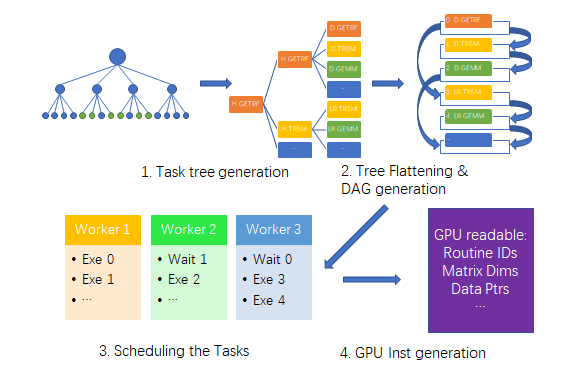
\includegraphics[width=\linewidth]{host_illust}
  \caption{An Illustration of the Host.}
  \Description{An Illustration of the Host.}
\end{figure}

\begin{itemize}

    \item {\verb|1. Task Tree Generation|}:
    
    CPU traverses the hierarchical matrix structure and determines the operations needed to be performed on each block to complete the LU factorization, without modifications on the actual data.
    
    \item {\verb|2. Tree Flattening & DAG Generation|}:
    
    Tree flattening takes the tree of tasks generated, and gets rid of intermediate hierarchical nodes which are fully represented by their dense and low-rank children. Data dependency checks are then performed between each task, and the result is stored as a DAG (Directed Acyclic Graph).
    
    \item {\verb|3. Scheduling the Tasks|}:
    
    With the tasks and their data dependency information, the scheduler uses 2 different heuristics to create a static scheduling: which task to fetch \& which worker to schedule to. Additional trimming and the estimated FLOPS are also used to assist the scheduler to further improve device utilization.
    
    \item {\verb|4. GPU Inst Generation|}:
    
    The last task of the CPU is translating the scheduling and the task information to the GPU correctly. Data pointers are batched together into an array, and BLAS-like and low-rank routines are enumerated. Along with the matrix dimensions and pointer offsets, each worker gets an integer array to represent the tasks being assigned to them.
    
\end{itemize}


\subsection{Device}

As all tasks are properly batched, there is no need for GPU to know the hierarchical structure, which implies no more recursion inside the kernel. In general, the kernel is made of 2 components: kernel level controlling functions and thread-block level routines. Additionally, warp-level intrinsics are used to optimize the thread-block level routines.

\begin{figure}[ht]
  \centering
  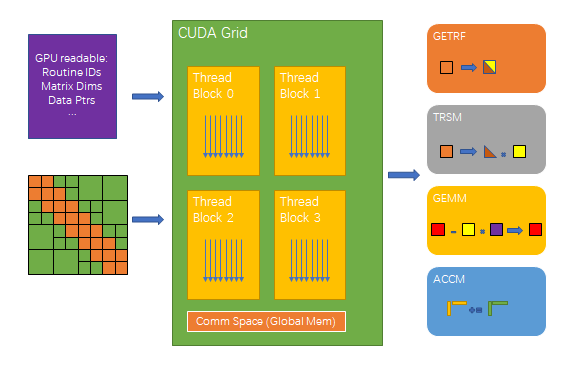
\includegraphics[width=\linewidth]{device_illust}
  \caption{An Illustration of the Device.}
  \Description{An Illustration of the Device.}
\end{figure}

On the kernel level, it is sometimes necessary to deliberately halt one or several SMs in order to correctly meet data dependency requirements until another SM finishes its work. However, as NVIDIA does not provide such functions in the CUDA programming model, we allocated space in the global memory as communication space for the SMs, and adopted a spin-lock mechanism. Instead of halting, SMs each assigns 1 thread that actively checks the state of the lock that it is waiting. In order to save the memory bandwidth, and possess minimal impact to other busy SMs, a waiting time hint is also provided by the CPU, correlating to the estimated FLOPS that needs to be completed. 

On the thread-block level, several BLAS-like routines and Low-rank routines are implemented as device functions in the kernel. Each device function takes all threads assigned to 1 SM to execute, and utilizes the full amount of shared memory and L1 cache. Inside each device function, vectorized memory I/O and warp shuffling techniques are used to further optimize each routines.

List of routines:

\begin{itemize}
    \item {\verb|GETRF|}: LU decomposition.
    \item {\verb|TRSM|}: Triangular solve of linear systems.
    \item {\verb|GEMM|}: General Matrix-matrix multiplication.
    \item {\verb|ACCM|}: Accumulation of low-rank blocks.
\end{itemize}

\section{Result}
When testing our code, we used double precision (FP64), constant rank 16, and a minimal block size of 256 x 256 for compression. Large low-rank blocks are partitioned deeper to at most N/8 x N/8 to increase task level parallelism. In general, without extreme tuning, we achieved satisfactory performance on a single GPU (NVIDIA Tesla V100 PCI-E 16GB), that can rival some well-optimized CPU-based hierarchical matrix libraries.

\begin{table}[ht]
  \caption{Pastel-Palettes, H-LU Performance}
  \begin{tabular}{ccccl}
    \toprule
    N & Flops & Host (ms) & Kernel (ms) & Kernel (GFlops)\\
    \midrule
    1024 & 3.027 E8 & 1.8 & 35.0 & 8.7\\
    2048 & 8.149 E8 & 3.3 & 71.0 & 11.5\\
    4096 & 2.440 E9 & 11.3 & 148 & 16.5\\
    8192 & 6.132 E9 & 53.9 & 302 & 20.3\\
    16384 & 1.519 E10 & 150 & 627 & 24.3\\
    32768 & 3.716 E10 & 472 & 1305 & 28.5\\
  \bottomrule
\end{tabular}
\end{table}

Hierarchical low-rank matrix compresses the total FLOPS for LU factorization needed to 0.158\% of the dense LU (2.346 E13 Flops, N=32768), which is equivalent to more than 15TFlops/s (from 28.5GFlops/s) if performed directly on a dense matrix.

\begin{figure}[ht]
  \centering
  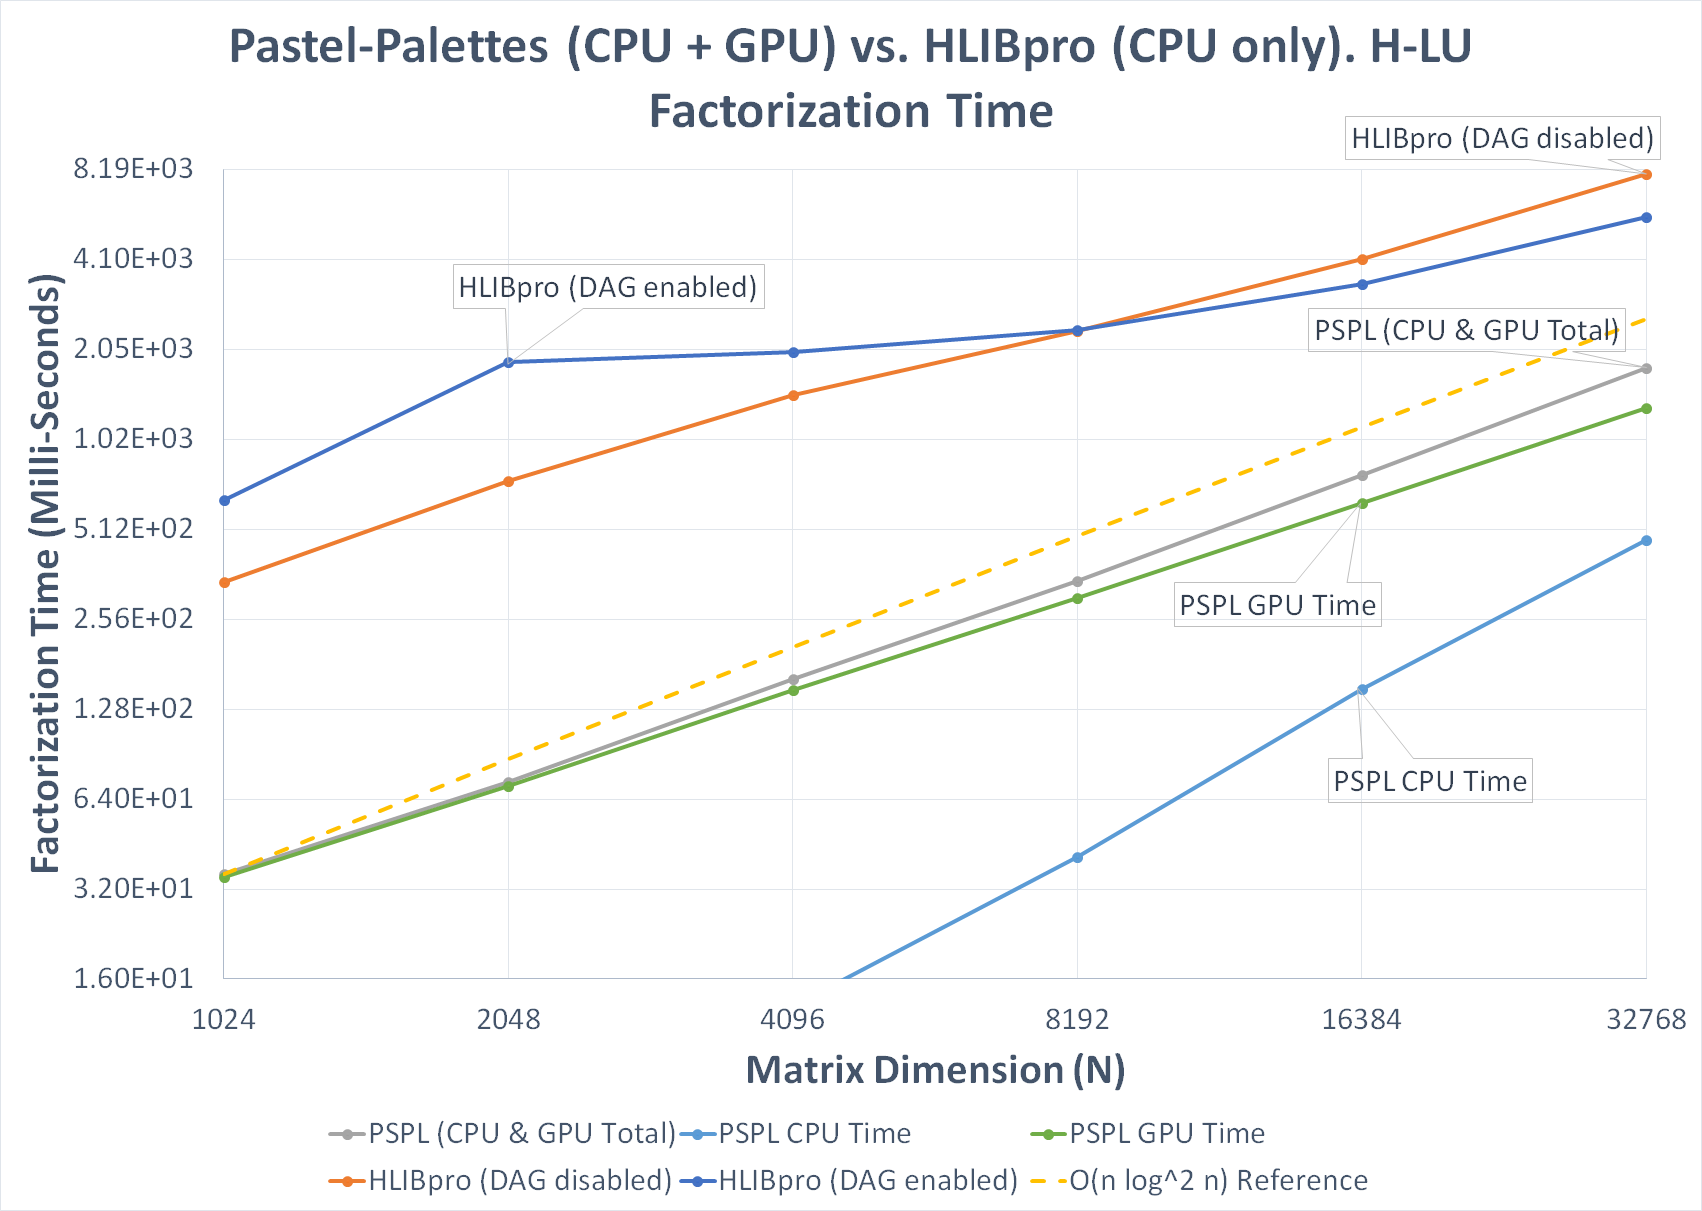
\includegraphics[width=\linewidth]{kernel_time}
  \caption{Pastel-Palettes vs. HLIBpro. H-LU Performance.}
  \Description{Pastel-Palettes vs. HLIBpro. H-LU Performance.}
\end{figure}

When comparing to existing H-matrix libraries, HLIBpro\cite{Kriemann13} also implemented task-based H-LU using only CPU. HLIBpro uses a well-tuned linear algebra library, LAPACK, for dense and low-rank routines. As the result shows, our implementation shows generally faster performance than HLIBpro, and the DAG overheads are less noticeable in the overall performance.

\section{Conclusion}
Conclusively, we discovered that although GPUs are typically considered ineffective handling tree structures and recursions, with enough preprocessing from the CPU, trees can be transformed into batched tasks effectively. Additionally, Hierarchical Low-rank Approximations of matrices compresses the FLOPS required for matrix calculations very significantly, which is not only LU factorization. We believe that our approach could be developed further to accommodate even more kinds of H-matrix calculations.

\begin{acks}
This work was supported by JST CREST Grant Number JPMJCR19F5.
\end{acks}

\bibliographystyle{ACM-Reference-Format}
\bibliography{sc}

\end{document}